%%%%%%%%%%%%%%%%%%%%%%%%%%%%%%%%%%%%%%%%%%%%%%%%%%%%%%%%%%%%%%%%%%%%%%%%%%%%%%%%%%%%%%%%%
% LICENSE NOTICE (CC BY 4.0)
%
% Author/Creator: Alexander Menzel
% Copyright: 2025 MitaTherm
%
% This work is licensed under the Creative Commons Attribution 4.0 International License.
% License Text (URI): https://creativecommons.org/licenses/by/4.0/
%%%%%%%%%%%%%%%%%%%%%%%%%%%%%%%%%%%%%%%%%%%%%%%%%%%%%%%%%%%%%%%%%%%%%%%%%%%%%%%%%%%%%%%%%

\chapter{Objectives and concept presentation}
\label{chap:Objectives and concept presentation}
%
The focus of presented master project is development of a modern software for a \ac{mcu}-based radiator thermostat and its commitment to public domain. The master project will be realized as a part of a bigger interdisciplinary development including:

\begin{itemize}
	\item \textbf{Mechanics}: Development of the thermostats power transmission for proper function with commonly used radiator valves, followed by design of an enclosure. This work will be presumably realized by Anton Surikov and advised by Prof. Dr. Tobias Müller.
	\item \textbf{Electronics}: Development of the thermostats \ac{pcb} and its integration with mechanical components, presumably realized by Thomas Schneider and advised by Prof. Dr. Daniel Schönherr.
	\item \textbf{Control algorithms}: Engineering of control algorithms to be used by the thermostat.
	\item \textbf{Software}: The subject of this work, development of the thermostats software and its integration with \acs{pcb} components. It will be presumably realized by Alexander Menzel and advised by Prof. Dr. Uwe Werner.
\end{itemize}

In the first part of this project a basic software for the device should be implemented including hardware drivers and state machines. At the end of this part a scientific paper will be written as an \ac{ieee} report.

The software should be designed ready for prospective integration of the control algorithms and \ac{ble}. The last feature is supposed to be used for smart home applications namely integration of the thermostat in Home Assistant and/or for provisioning of a \ac{http} \ac{api} using a gateway.

Following points are consequently objectives of this master project:

\begin{itemize}
	\item Development or integration of drivers for all radiator thermostat components.
	\item Development of basic consumer functions.
	\item Writing of a \acs{ieee} report describing program design.
\end{itemize}

\newpage

\begin{figure}[p]
	\centering
	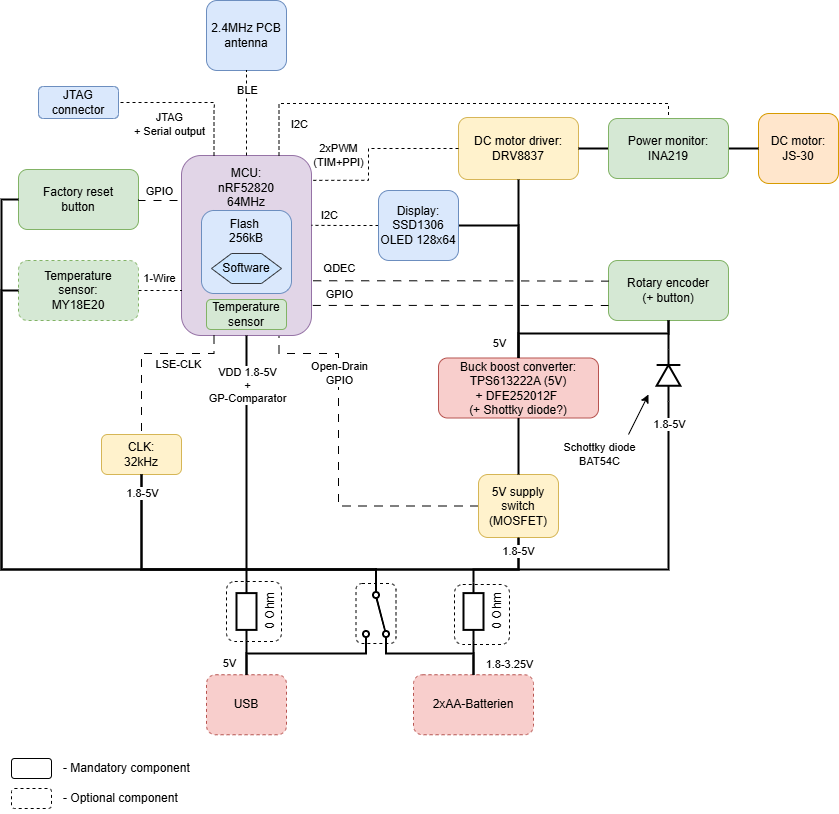
\includegraphics[width=1.0\linewidth]{../../electronics/mt-rt-block-diagram.png}
	\caption{Current version of the block diagram for the radiator thermostat (draft)}
	\label{fig:mt-rt-block-diagram}
\end{figure}

\newpage

